An is interrupt triggered for every commutation high and the ISR gets the counter
value of an independently runing timer. Using this value, the RPM is calcluated
at every interrupt trigger as follows:
\begin{align*}
    rpm &= \frac{60 f_t}{N_p \times T_c}\\
    \text{Where,} \qquad &\\
    f_t &- \text{Frequency of the timer counts (here, $1$ MHz)}\\
    N_p &- \text{Number of pole-pairs in the BLDC motor (here, $7$)}\\
    T_c &- \text{Timer counts between the two interrupts}
\end{align*}

The above method of measurement is verified against the tach-meter reading. The
readings are in agreement with each other, validating the measurement method.
\begin{figure}[H]
    \centering
    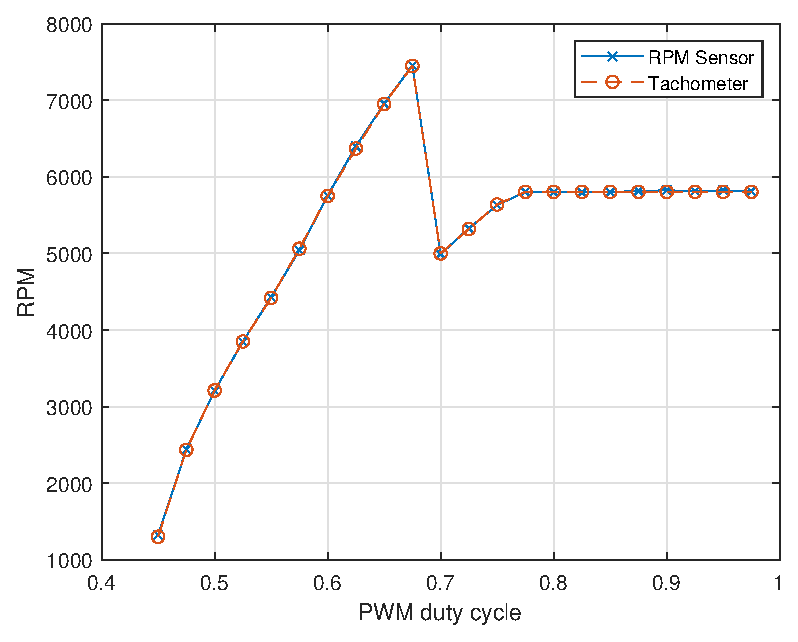
\includegraphics[width=0.5\textwidth]{./figs/rpm_feedback/static_calib.eps}
    \caption{Rpm sensor and tachometer readings}
\end{figure}

The above method has an inherent flow at very low $rpm$s where there is no
commutation at a given sampling instance which results in a zero rpm at that
sample making the sensor noisy. This can be avoided by holding the rpm value
from the previous measurement if there is no commutation in the sample instance.

\bigskip

\itbf{Using external interrupt and  timer}
\par The commutations can be counted using external interrupts. The actual measurement of rpm involves a raising-edge triggered external interrupt and a timer interrupt. The ISR of the external interrupt updates a counter corresponding to the pulses (here, the electrical commutations). The timer-interrupt polls for this counter value at the specified frequency $(f_s)$ and resets the counter. The rpm is calculated from this counter value as follows:
$$rpm = \frac{counter\_value}{N_P} \times f_s \times 60$$
where, \\
$N_p - $ No. poles in the BLDC motor\\

\par The minimum rpm that can be measured depends on the sampling frequency and the poles in the BLDC motor $(= \frac{60f_s}{N_P} )$. And the maximum depends on the clock frequency of the micro-controller as the frequency of interrupts and ISR calls becomes the bottleneck in this case. The resolution of the sensor also depends on the sampling frequency and poles as the counter value is an integer. We have,
$$Sensor \, resolution = \frac{60f_s}{N_P}$$

\par For the current system the range of rpm is $[2000, 10000]$. The number of poles in BLDC motor are $12$. Assuming the acquisition frequency of $400\,Hz$, the resolution for the above sensor will be:
$$Sensor \, resolution = \frac{60f_s}{N_P} = 2000 \, rpm = 209.4395 \, rad/s$$
For $100 \, Hz$ acquisition rate:
$$Sensor \, resolution = 500 \, rpm = 52.3599 \, rad/s$$

\par The main source of sensor noise in this case is the latency of the external interrupt. The counter value will be oscillating around the actual value based on the timing of external and timer interrupts causing the measured rpm to fluctuate. Based on the resolution calculations above, the signal-to-noise ratio of the system will be very high if the current implementation is used. \\

\par This problem of resolution and signal-to-noise ratio is due to the interfacing method used. Alternatively, the following method is propsoed to overcome this problem.

\bigskip

\itbf{Using two timers and an external interrupt}
\par We use and additional timer as a high frequency counter of frequency $f_t$ for calculating the rpm at every sampling period as follows:
$$rpm = \frac{counter\_value \times f_t}{N_P \times time\_counts} \times 60$$
where, \\
$N_p - $ No. poles in the BLDC motor\\
$time\_counts - $ Number of timer interrupt counts during the sampling interval.\\
Hence, we have, maximum number of $time\_counts$ in a sampling interval is $f_s/f_t$\\
$$\implies Sensor \, resolution = \frac{60f_s}{N_P f_t} = rpm_{min}$$
Therefore, the resolution of the sensor can be increased by arbitrarily increasing the frequency of the high frequency counter, limited only by the hardware.\\

For example, if $f_h = 1000\, Hz$, for the same values as above, the resolution of the sensor:
$$Sensor \, resolution = \frac{60f_s}{N_P \times f_t} = \frac{2000}{1000} = 2 \, rpm = \frac{1}{\pi} \, rad/s$$

\par This method will reduce the signal-to-noise ratio significantly.

\subsection{Measurement Algorithm}
\par In higher rpm cases there are more than one measurement instance wthin
the sample time. Median of these measurements can be used to reduce sudden spikes in the data due to interrupts skips. Combining this with
higher resolution algorithm, we have the algorithm for rpm measurement:\\

Let $C_c$ be the current value of the 32-bit timer, $P_c$ the previous value and $n_C$ be the number of commutations within the sample.\\

At every interrupt trigger (in ISR)

    \begin{algorithm}[H]
        $n_C \peq 1$\;
        $\delta t_k = C_c - P_c$\;
        \If{ $\delta t_k \leq 0$ }
            {$\delta t_k \peq 2^{32}$ \Comment*[r]{Correcting for integer overflow}}
        $\pmb{\delta t_k} [n_C-1] =  \delta t_k$\;
        $P_c = C_c$\;
    \end{algorithm}

At every sampling instance (in $get\_rpm()$):

    \begin{algorithm}[H]
        $N_p = 7$\;
        $f_t = 10^6$\;
        $M = \frac{2 \pi}{N_p} \times f_t$\;
        \eIf {$n_C > 0$ and $n_C \leq n_{C_{max}}$ and $\norm{n_C - n_{C_{old}}} \leq \delta n_{C_{max}}$}
            {$\omega = \frac{M}{\text{Median}(\pmb{\delta t_k})}$ \Comment*[r]{Median removes spikes in the data}
             $ \omega_{old} = \omega$\;
             $n_{C_{old}} = n_C$\;
            }
             {$\omega = \omega_{old}$}
        $n_C = 0$\;
        $\pmb{\delta t_k} = \pmb 0$\;
    \end{algorithm}

\begin{figure}[H]
    \begin{minipage}{0.49\textwidth}
        \begin{figure}[H]
            \centering
            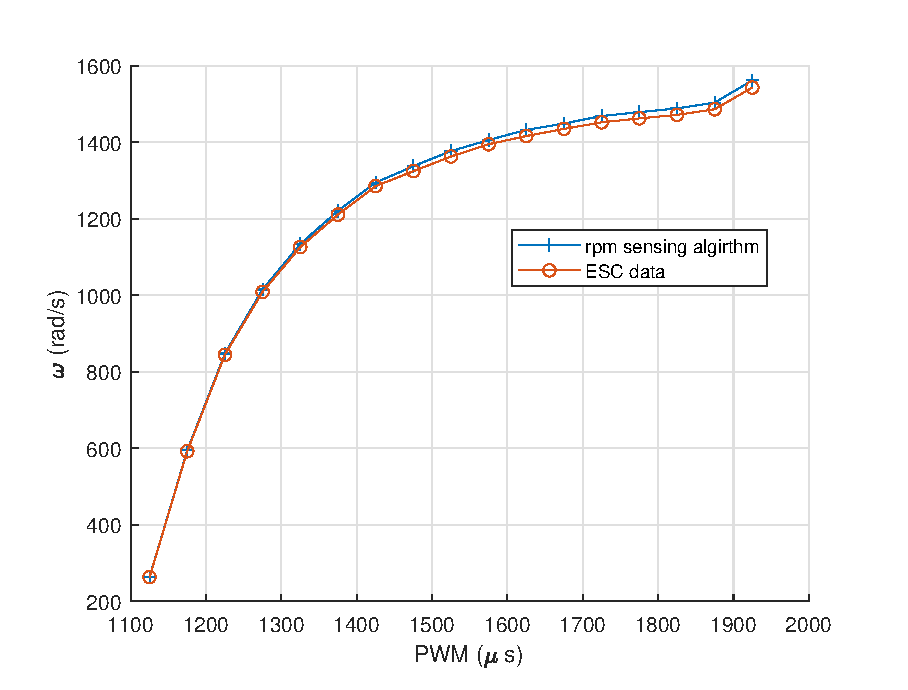
\includegraphics[width = \textwidth]{./figs/rpm_feedback/rpm_meas_noprop.eps}
            \caption*{Without Propeller}
        \end{figure}
    \end{minipage}
    \begin{minipage}{0.49\textwidth}
        \begin{figure}[H]
            \centering
            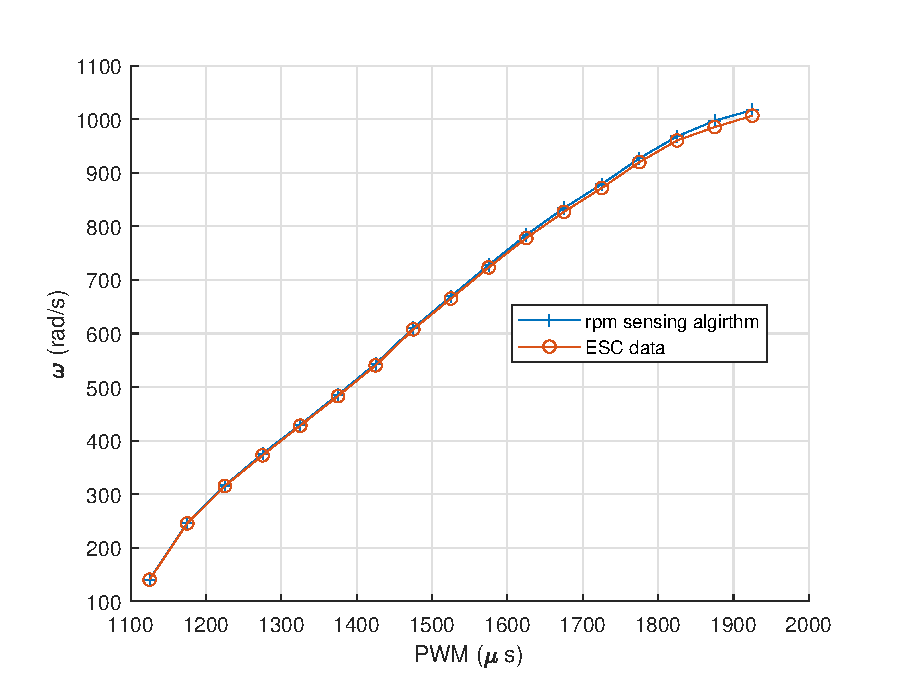
\includegraphics[width = \textwidth]{./figs/rpm_feedback/rpm_meas_prop.eps}
            \caption*{With Propeller}
        \end{figure}
    \end{minipage}
    \caption{Validating the measurement algorithm}
\end{figure}
